% Source: graduate-coursework/Research/Intro_to_Agents/handouts/Part2_Agent_Foundations.tex

\documentclass[border=4pt]{standalone}
\usepackage{amsmath}
\usepackage{amssymb}
\usepackage{tikz}
\usepackage{xcolor}
\usetikzlibrary{shapes.geometric, arrows.meta, positioning, fit, calc, backgrounds}

\definecolor{UofSCGarnet}{HTML}{73000a}
\definecolor{UofSCBlack}{HTML}{000000}
\definecolor{UofSCWhite}{HTML}{ffffff}
\definecolor{UofSCAtlantic}{HTML}{466A9F}
\definecolor{UofSCCongaree}{HTML}{1F414D}
\definecolor{UofSCRose}{HTML}{CC2E40}
\definecolor{UofSCHorseshoe}{HTML}{65780B}
\definecolor{UofSCGrass}{HTML}{CED318}
\definecolor{UofSCHoneycomb}{HTML}{A49137}
\definecolor{UofSCDarkGarnet}{HTML}{570008}
\definecolor{UofSCAzalea}{HTML}{844247}
\definecolor{UofSC90Black}{HTML}{363636}
\definecolor{UofSC70Black}{HTML}{5C5C5C}
\definecolor{UofSC50Black}{HTML}{A2A2A2}
\definecolor{UofSCWarmGrey}{HTML}{676156}
\definecolor{UofSCSandstorm}{HTML}{FFF2E3}

\tikzset{
    % Box styles with sharp corners
    component/.style={
        rectangle,
        draw=UofSCBlack,
        fill=UofSCWhite,
        thick,
        minimum width=3cm,
        minimum height=1cm,
        align=center,
        font=\small
    },
    component garnet/.style={
        component,
        fill=UofSCGarnet!10,
        draw=UofSCGarnet,
        thick
    },
    component atlantic/.style={
        component,
        fill=UofSCAtlantic!10,
        draw=UofSCAtlantic,
        thick
    },
    component congaree/.style={
        component,
        fill=UofSCCongaree!10,
        draw=UofSCCongaree,
        thick
    },
    loop node/.style={
        rectangle,
        draw=UofSCGarnet,
        fill=UofSCGarnet!15,
        thick,
        minimum width=2.5cm,
        minimum height=1.2cm,
        align=center,
        font=\footnotesize\bfseries
    },
    decision/.style={
        diamond,
        draw=UofSCBlack,
        fill=UofSCHoneycomb!20,
        thick,
        minimum width=2cm,
        minimum height=1.5cm,
        align=center,
        font=\footnotesize,
        aspect=2
    },
    arrow style/.style={
        ->,
        >=Stealth,
        thick,
        UofSCBlack
    },
    biarrow style/.style={
        <->,
        >=Stealth,
        thick,
        UofSCBlack
    }
}

\begin{document}
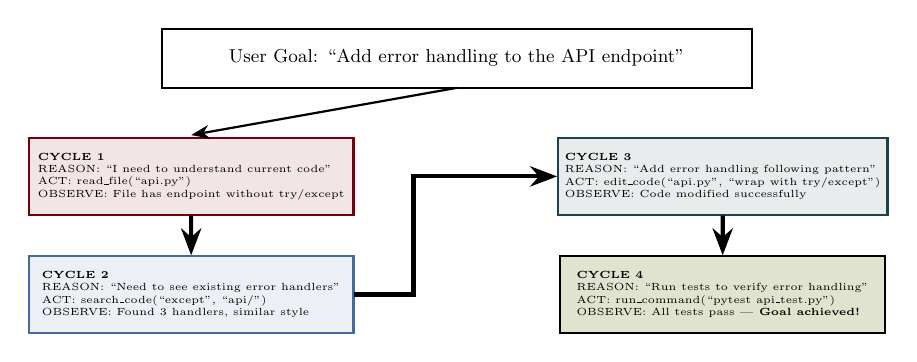
\begin{tikzpicture}[scale=0.75, transform shape]
        % Cycle 1
        \node[component garnet, minimum width=5.5cm, minimum height=1.3cm, align=left, font=\tiny] (c1) at (-4.5, 2.5) {
            \textbf{CYCLE 1}\\
            REASON: ``I need to understand current code''\\
            ACT: read\_file(``api.py'')\\
            OBSERVE: File has endpoint without try/except
        };

        % Cycle 2
        \node[component atlantic, minimum width=5.5cm, minimum height=1.3cm, align=left, font=\tiny] (c2) at (-4.5, 0.5) {
            \textbf{CYCLE 2}\\
            REASON: ``Need to see existing error handlers''\\
            ACT: search\_code(``except'', ``api/'')\\
            OBSERVE: Found 3 handlers, similar style
        };

        % Cycle 3
        \node[component congaree, minimum width=5.5cm, minimum height=1.3cm, align=left, font=\tiny] (c3) at (4.5, 2.5) {
            \textbf{CYCLE 3}\\
            REASON: ``Add error handling following pattern''\\
            ACT: edit\_code(``api.py'', ``wrap with try/except'')\\
            OBSERVE: Code modified successfully
        };

        % Cycle 4
        \node[component, fill=UofSCHorseshoe!20, minimum width=5.5cm, minimum height=1.3cm, align=left, font=\tiny] (c4) at (4.5, 0.5) {
            \textbf{CYCLE 4}\\
            REASON: ``Run tests to verify error handling''\\
            ACT: run\_command(``pytest api\_test.py'')\\
            OBSERVE: All tests pass --- \textbf{Goal achieved!}
        };

        % Arrows
        \draw[arrow style, line width=1.5pt] (c1) -- (c2);
        \draw[arrow style, line width=1.5pt] (c2.east) -- ++(1,0) |- (c3.west);
        \draw[arrow style, line width=1.5pt] (c3) -- (c4);

        % User goal at top
        \node[component, minimum width=10cm] at (0, 4.5) {User Goal: ``Add error handling to the API endpoint''};
        \draw[arrow style] (0, 4) -- (-4.5, 3.2);
    \end{tikzpicture}
\end{document}
